% Auto-generated robustness figures
\begin{figure}[h]
  \centering
  % Use paths relative to paper/ directory for portability; break lines to avoid overflow
  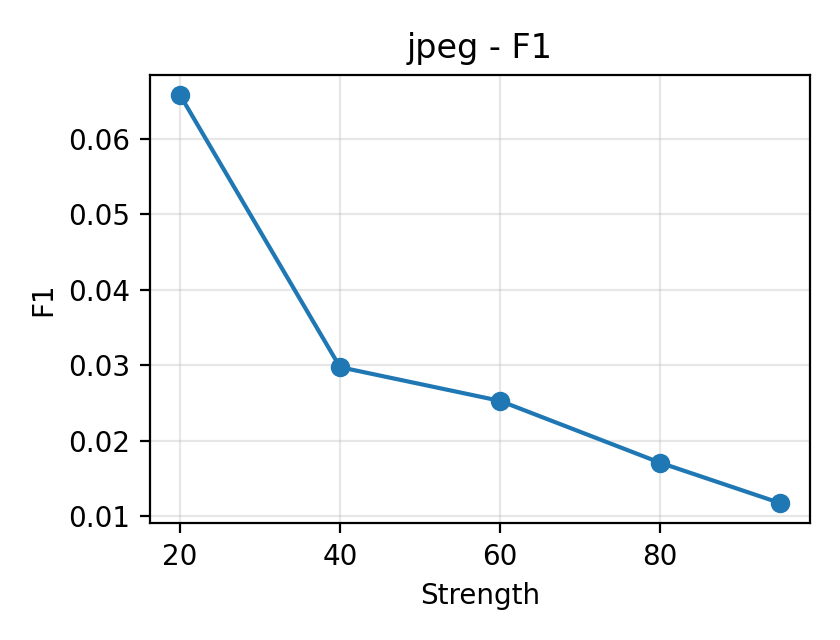
\includegraphics[width=.32\textwidth]{figures/figures_outputs_stage5_robustness_jpeg_f1.png}% jpeg
  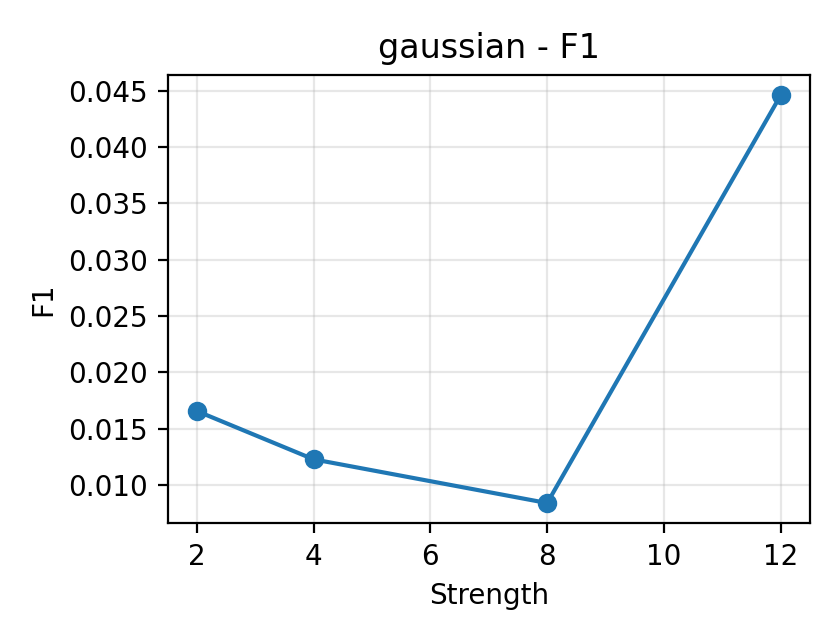
\includegraphics[width=.32\textwidth]{figures/figures_outputs_stage5_robustness_gaussian_f1.png}% gaussian
  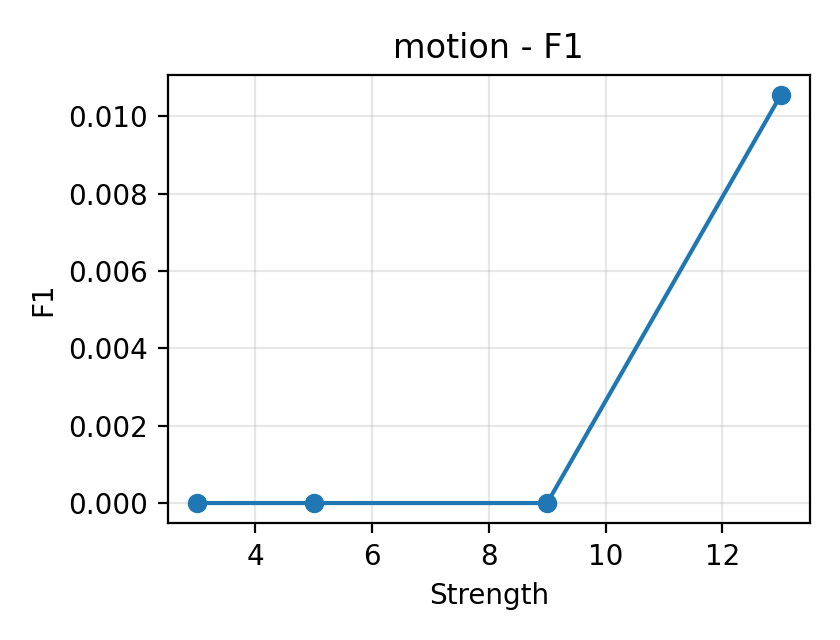
\includegraphics[width=.32\textwidth]{figures/figures_outputs_stage5_robustness_motion_f1.png}% motion\\
  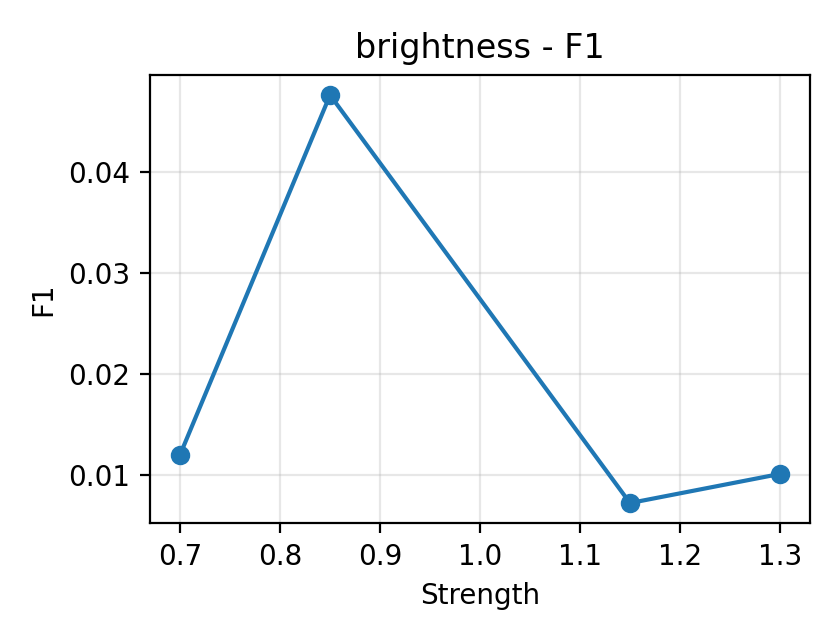
\includegraphics[width=.32\textwidth]{figures/figures_outputs_stage5_robustness_brightness_f1.png}% brightness
  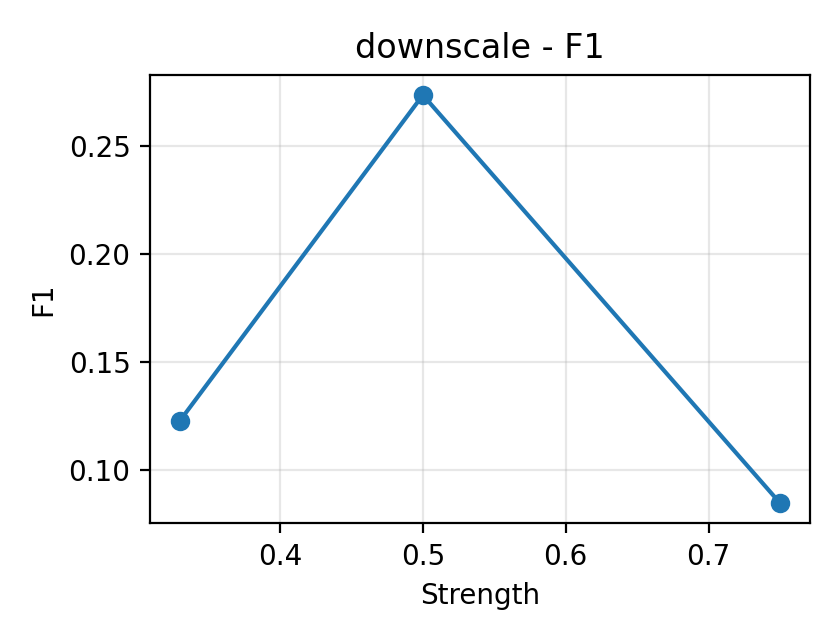
\includegraphics[width=.32\textwidth]{figures/figures_outputs_stage5_robustness_downscale_f1.png}% downscale
  \caption{Robustness: metric curves under common perturbations.}
  \label{fig:robustness_curves}
\end{figure}
